\section{Management Approach}

This collaborative effort is in part to advance our understanding of
the bio-geophysical processes in the \naz area, while advancing the
observational technology and capacity in the coastal ocean.  \proj
will be managed by the PI (Rajan, a US national) working closely with
the collaborators from the \texttt{Univ.~of Porto}, \texttt{Instituto
  Hidrogr\'{a}fico}, \texttt{Univ.~of Aveiro}, \texttt{Columbia
  Univ.}, \texttt{MIT} and \texttt{SOCIB}.  All key personnel have
known and worked with one another, most over a decade, some at
sea. \univ will be the prime, where the PI has a Visiting Professor
position. 

\begin{table}[!t]
  \centering
  % \vspace{-0.5cm}
  \footnotesize{
  \begin{tabular}{|p{2.7cm}|p{2.5cm}|p{5cm}|p{4.5cm}|}\hline 
    \rowcolor{Gray}
    \bfseries Name& \bfseries Institution&\bfseries Expertise/Qualification &\bfseries Contributions\\
    \hline
    Kanna Rajan&\orge, US and \texttt{Univ. of Porto}, Portugal&PI, Autonomy, Adaptive Sampling&Organization, reporting, experiment design, outreach\\
    \hline
    Jo\~ao Sousa&\texttt{Univ. of Porto}, Portugal&Co-PI, Operations Lead, CONOPS (concept of operations) design and
            implementation, software eng.
                                    &Organization, Aerial/surface/underwater
                                      vehicles, comms\\
    \hline
    Jo\~ao Vitorino&\texttt{Instituto Hidrogr\'{a}fico},
                     Portugal&Physical Oceanography,
                               Modeling&Observation assimilation and modeling,
                                         CONOPS, prediction, local outreach\\
    \hline
    Marina Cunha&\texttt{Univ. of Aveiro}, Portugal&Coastal Ecology&Biological sampling, lab analysis\\
    \hline
    Joaqu\'{i}n Tintor\'{e}&\texttt{SOCIB}, Spain &Physical Oceanography &Experiment
                                                          design,Gliders and operations\\
    \hline
    Ajit Subramaniam&\texttt{Columbia Univ.}, US&Biological Oceanography&CONOPS, sampling
                             algorithms\\
    \hline
    Pierre Lermusiaux&\texttt{MIT}, US&Modeling, Machine Learning and entropy
                             reduction&Modeling support\\
    \hline
  \end{tabular}
  \caption{Roles and responsibilities and in-kind contributions in
    \proj for the proposed 2021 Sept-Oct field experiment. All team
    members will be collaboratively involved in experiment design and
    post experiment publishing.}
  \label{tab:roles}
}
\end{table}

\paragraph{Roles and responsibilities} \univ will be the lead
organization, provide aerial, surface and underwater vehicles,
communication equipment and command/control software while
coordinating all activities. Funding requested will primarily support
students and staff in Porto for the period of the experiment for
$\sim 20$ days. \inst will provide the assimilation, modeling and
prediction with shore-side models. In addition \inst will conduct CTD
and vessel mounted observations onboard the research vessel and also
provide access to their research vessel as well as a RHIB or rigid
boat. \mit will support \inst for \texttt{HOPS} modeling and
augmentation for ML capabilities. \colo and \ave will work on making
bio-optical and biological measurements and providing analysis and
data to augment \inst modeling. Table \ref{tab:roles} summarizes the
roles and contributions of all partners. \soc will provide a glider
and personnel for preparation, deployment, operations and support of
the vehicle as well as helping with the analysis of glider data during
and after the experiment. The roles and responsibilities of the key
personnel are summarized in Table \ref{tab:roles}.


\paragraph{Budget Request} Our funding request is highly leveraged
with equipment and people who are keen on participating in this
experiment. No salaries, or expensive ship-times are being requested,
instead we will be using existing assets which will be in the \naz
area for fixed periods of time and use robotic hardware and software
from \univ and \soce. Consequently, our budget reflects costs for
consumables, insurance, SatComs, and travel only. \univ is the primary
beneficiary of this request with minor requests for \inste, \avee,
\colo and \soc (Table \ref{tab:budget}). No funding is being
requested for \mite.

\begin{table}[!t]
  \centering
  % \vspace{-0.5cm}
  \footnotesize{
  \begin{tabular}{|p{3.3cm}|p{1.3cm}|p{1.4cm}|p{8cm}|}
    % \multicolumn{1}{l}{r}{l}
    \hline 
    \rowcolor{Gray}
    \bfseries Item& \bfseries Inst.&\bfseries Cost (\$) &\bfseries Comment\\
    \hline
    Small-boat rental&\univ&16,958&19-day rental\\
    \hline
    Semi-rigid small-boat&\inst&1,785&\inst small-boat transported
                                       from Lisbon for ops with
                                       research vessel\\
    \hline    
    Insurance (AUVs)&\univ&31,654&Insurance costs for 7 AUVs\\
    \hline
    Insurance (UAVs)&\univ&1,190&Insurance costs for 2 UAVs\\
    \hline
    Lodging&\univ&7,616&Costs for lodging in \naz area 8 personnel for 20 days\\
    \hline
    Subsistence&\univ&11,424&Costs for subsistence in \naz area for 8
                              personnel for 20 days\\
    \hline
    Communication costs&\univ&11,870&SatComs for AUVs for 19
                                      operational days\\
    \hline
    Rental Cars&\univ&7,140&Rental cars/vans for transporting
                             equipment from Porto\\
    \hline
    Gas \& Tolls&\univ&1,179&\\
    \hline
    Consumables&\univ&10,710&Short lifetime needs for field operations
                              with autonomous platforms such as
                              batteries, fins, servo-motors for the
                              rudders, bolts, o-rings, etc\\ 
    \hline    
    Cellular Comms&\univ&893&\\
    \hline    
    Sample Processing&\ave&5,950&Biological water sample processing
                                  during and post-experiment\\
    \hline    
    Sample Processing&\inst&1,190&Consumables for BGC water sample
                                   analysis at \inst\\
    \hline    
    Glider batteries&\soc&3,570&Consumables for glider ops\\
    \hline
    Glider comms&\soc&4,760&Iridium SatCom costs for glider ops\\
    \hline    
    Travel from US&\colo \& \org&4,046&Travel from US and lodging for
                                         Subramaniam \& Rajan\\
    \hline
    \multicolumn{1}{|r|}{\textbf{Total}}&&121,933&\\
    \hline    
  \end{tabular}
  \caption{Budget details for \proj field experiment in USD.}
  \label{tab:budget}
}
\end{table}

\subsection{\proj Operations}
 
% Real-time monitoring systems:

\begin{wrapfigure}{!h}{3.0in}
  \vspace{-0.8cm}
  \centering
  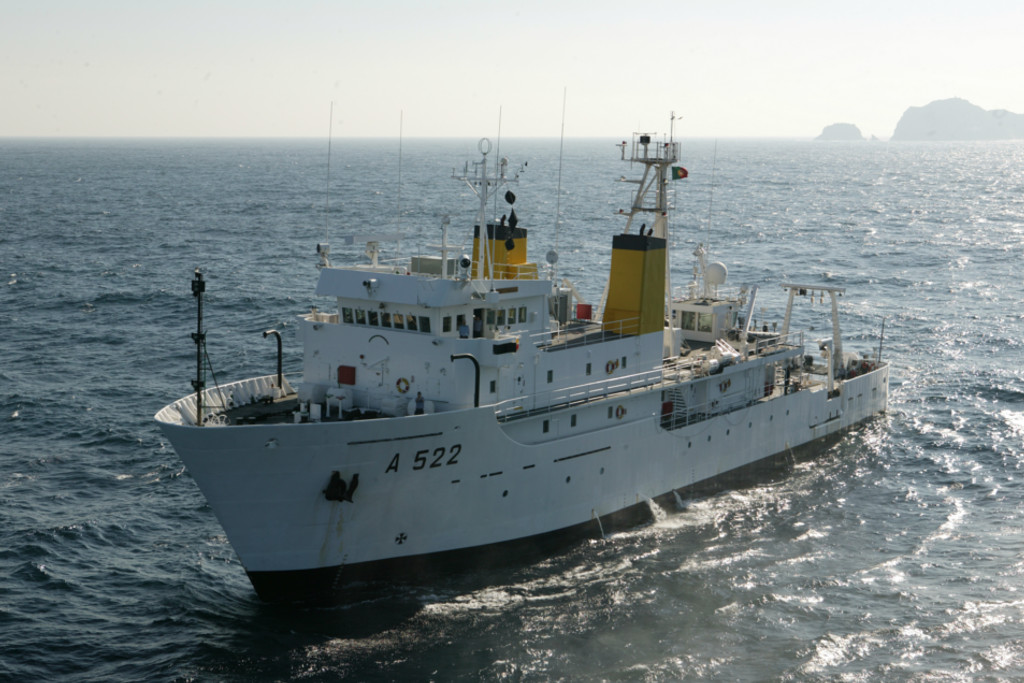
\includegraphics[scale=1.75]{fig/dom-carlos.jpg}
  \caption{A 70m research vessel, the NRP \emph{Dom Carlos} or its
    sister vessel will be available for \proje.}
  \vspace{-0.3cm}
 \label{fig:vessel}
\end{wrapfigure}

Off shore in the \naz canyon-Berlengas area are two islands of Berlengas
and Farilho\~es part of a protected nature preserve. With special
permission we expect to be able to be based in Berlengas for a period of
3 weeks to conduct off shore operations. A small team will also be
present onboard the \inst research vessel where if needed, deployment
and recovery of assets well off shore at the boundaries of the survey
region, can be done. In addition \inst will be in a position to provide
a RHIB or a rigid boat for near-shore operations from the two islands.

\univ will provide the bulk of the robotic assets including aerial,
surface and underwater vehicles as also the team to operate them. The
team will be split between being based in Berlengas, the research vessel
and also provide remote monitoring from Porto. \soc will provide at
least one glider to operate outside the shelf to augment model
observations in the meso-scale.

\proj will leverage existing real-time monitoring capacities which were
installed and are operated by Instituto Hidrogr\'{a}fico (\inste). These
include two multi-parametric buoys with satellite transmission of hourly
data sets and two coastal tide gauges installed in the ports of \naz and
Peniche. These systems form the \naz Canyon Observatory \texttt{MONICAN}
which is a subset of the global real-time monitoring infrastructure for
the Portuguese Exclusive Economic Zone operated by \inst \kc{(MONIZEE
  infrastructure, see figure X)}. In addition, we will leverage ship
time from one of the \inst research vessels which visit the \naz area
for buoy maintenance twice yearly. \inst will provide access to this
vessel where a small \proj team will be resident, in addition to those
being housed in the Berlengas island.

Each multiparametric buoy is equipped with:

\begin{enumerate}[noitemsep,topsep=0pt,parsep=0pt,partopsep=0pt]

  \item A meteorological mast providing hourly measurements of wind speed and
    direction, air temperature, atmospheric pressure and relative
    humidity

  \item A wave sensor providing hourly measurements of standard wave parameters
    (wave spectra at the end of the deployment)

  \item A downward looking 300 kHz RDI Workhorse ADCP installed at 7 m
    depth and providing currents with $sim 2$ m resolution to about 90 m
    depth Surface temperature sensor (SBE AADI Subsurface temperature
    sensors)

\end{enumerate}  


The buoys are also equipped with fluorometers but the response of these
sensors rapidly degrades in about 1-2 weeks, after maintenance,
primarily due to biofouling.

Additional systems could also be available for \proje. A separate
project proposal was submitted at the end of 2020~\footnote{EEA Grants,
  Portugal} where a HF radar system has been proposed for the \naz area.
The system, a CODAR Seasonde with two antennas operating at 13 MHz, one
installed in \naz and the other in Peniche. A previous test of a similar
system was conducted by \inst in September--November 2011 and showed
that surface currents measurements were available for the complete area
to about 70 km from the shore with a 1 km resolution \kc{(figure)}.
 
  
\subsection{At-Sea operations}

\proj will observe the coastal ocean area of interest off of \naze, in
such a way as to improve the initialization/assimilation fields and
parameter definitions to be used in the physical and biogeochemical
models. To achieve this objective \proj will develop a strategy largely
inspired by the Rapid Environmental Assessment to navy operations
\kc{citation?}. Specifically a total of three phases (weeks 1 to 3) are
planned:


\begin{figure}[!t]
  \vspace{-0.5cm}
  \centering
  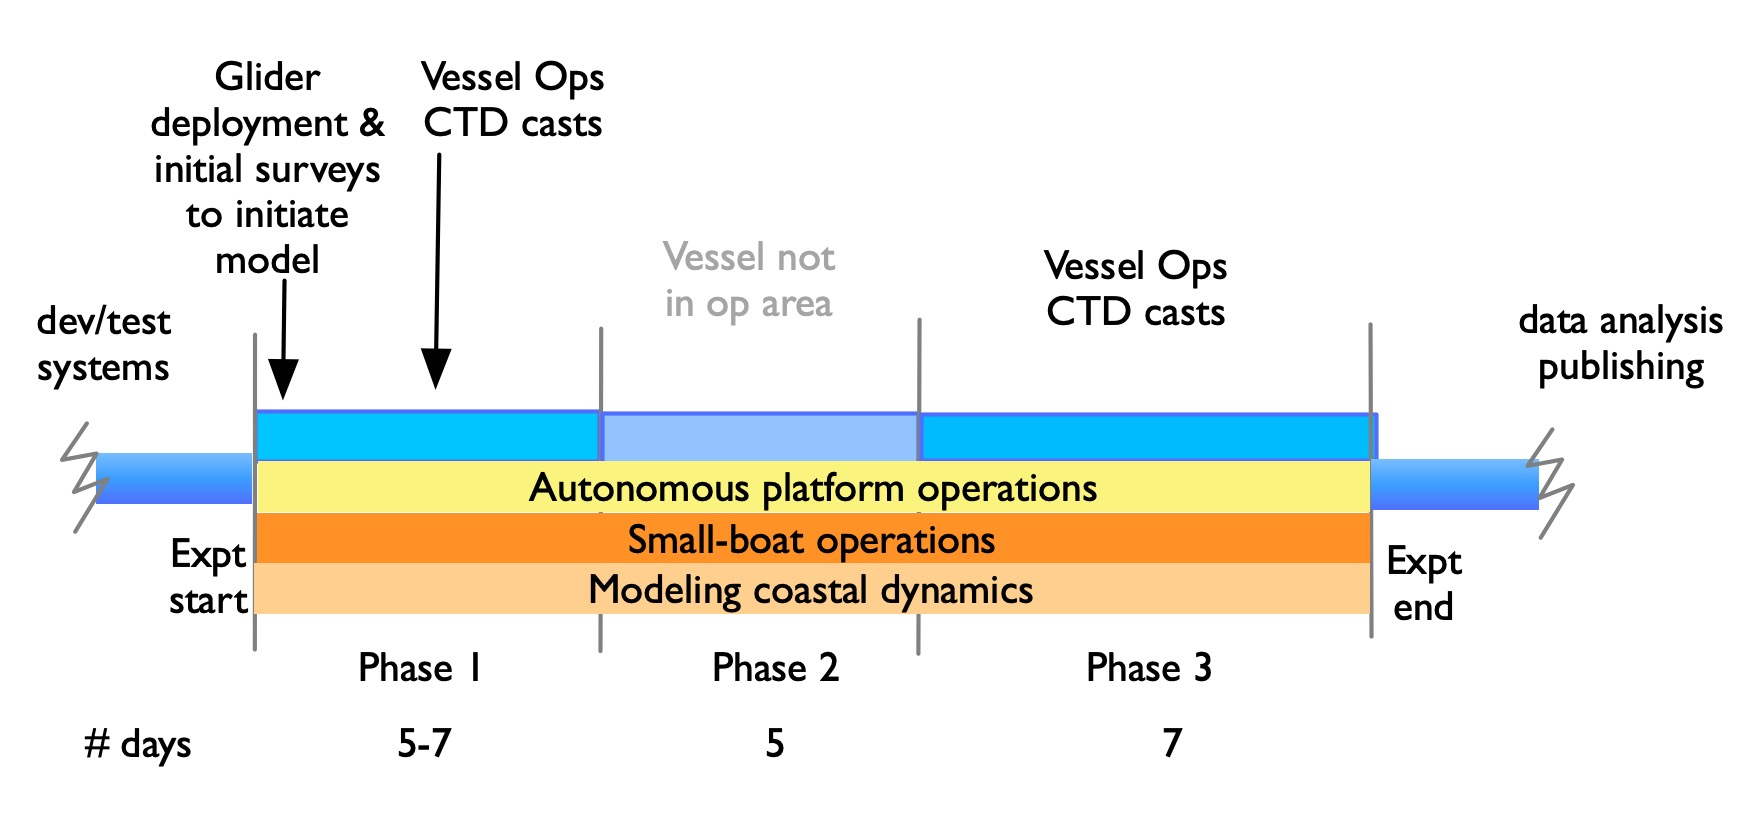
\includegraphics[scale=0.25]{fig/timelines.jpg}
  \caption{At-sea operations for \proj will be split along 3 phases.
    Phase 1 will involve glider deployments at the further reaches of
    the operational boundary, deployment of other autonomous platforms
    to initialize the model, calibrate sensors with limited ship based
    CTD casts. Phase 2 will commence when the vessel departs the \naz
    operational area. Phase 3 will commence with the resumption of
    vessel ops in the \naz area. Autonomous platforms starting with
    gliders will be operating continuously to target adaptive sampling
    driven by model predicts, through all phases.}
  \vspace{-0.3cm}
 \label{fig:expt-phases}
\end{figure}

 
% Phase 1 (precursor survey):
\paragraph{Phase 1} A preliminary characterization of the geographical
area of interest will be conducted during this phase with the
identification of the prevailing features that characterize the coastal
ocean area of \naz from remote sensing imagery and (if available) from
surface currents measured by HF radar. The data will allow
identification in SST, Chl, turbidity and currents, for example, and to
select a limited number of key stations which can be complemented by CTD
casts. % In case no surface data is
% available (because of cloud cover obstructing optical remote sensing)
% the location of these points will be dictated by the characteristics of
% the topography of the area, by the prevailing forcing conditions and by
% previous knowledge about the primary processes.
This phase will combine operations from small boats with operations
conducted onboard a \inst hydrographic vessel that will pass through the
area. Glider deployments off-shore to provide boundary conditions for
the models will be initiated and augment available remote sensing (or HF
radar) data. Sampling with vertical nets will also be done at some
stations; part of the water samples collected will be used to evaluate
the nutrient profiles in the water column. % These samples will be
% analyzed at the \inst Marine Chemistry and Pollution laboratories and
% will be available in about 1--2 days.
They will aid in characterizing the nutrient intake to upper levels
associated with intensified upwelling at the canyon head or the inputs
to the coastal ocean associated by freshwater inputs along the coast as
a means to initialize the nutrient fields in the BGC model. Analysis of
water samples collected by the small boats will be used for calibration
of the CTD fluorometer and as also to calibrate the ADCP echo intensity
data for zooplankton biomass. Remote operations from Porto will also be
tested as a means to demonstrate an Ocean Space Center (OSC)
\cite{lima21}. This phase will likely be between 5--7 days.

% During 2--3 days a team onboard a small-boat will conduct a set of
% measurements in the water column (to about 200 m depth) at the key
% location point identified earlier using low cost systems \kc{this is
%   vague} and other sensors of interest and water samples collected at
% selected depths on those key locations. Sampling with vertical nets will
% also be done at some of these positions. Part of the water samples
% collected will be used to evaluate the nutrient profiles in the water
% column. These samples will be analyzed at the \inst Marine Chemistry and
% Pollution laboratories and will be available in about 1--2 days.
% Depending on the period selected for the exercise these measurements
% would help to characterize the nutrient intake to upper levels
% associated with intensified upwelling at the canyon head or the inputs
% to the coastal ocean associated by freshwater inputs along the coast.
% Combined with the information available from remote sensing images, this
% data will provide the basis for the initialization of the nutrients
% fields in the BGC model.
 
% Part of the water samples and samples collected with a vertical net will
% be used to characterize the phyto- and zoo plankton communities. These
% samples will provide the basis for the initialization of the phyto and
% zooplankton compartments of the BGC model.
 
% At the same time the hydrographic vessel will pass on the area and
% during this period will conduct a very limited number of CTD profiles
% and collect vessel mounted ADCP measurements. The analysis of water
% samples collected by the small boat campaign at a few locations and same
% times will then be used for calibration of the CTD fluorometer and
% calibrate the ADCP echo intensity data in zooplankton biomass. These
% calibrations will then be used during next phase of the survey

% \kc{
% This data will also be used to calibrate the response of fluorometers to
% be used in response
 
% This phase will provide key points to be used in the following stages
% such as vertical profiles of temperature and salinity and water samples
% collected at selected depths to be used in the definitions of d
% will be inspired in the strategies used with real and assimilation
% fields. In \proj we propose to extend this This phase will provide the
% background knowledge to be used in the numerical model initialization
% such as and the definition of some of the basic parameters (such as
% light attenuation parameters and so one).. Also during this phase we
% calibrate the response of the some of the sensors using}
 
\paragraph{Phase 2} This phase will rely only on small boat operations
with the departure of the research vessel and provide additional
opportunities to fine tune the adaptive sampling algorithms, model
predictions and BGC model fields. Glider operations will continue to
provide updates to boundary conditions in the model even as other
autonomous platforms will continue to operate in a more constrained
field of scientific interest. Small boat operations will be from
Berlengas or \naz itself, especially for launch and recovery operations.
Monitoring autonomous platforms from remote shore-side locations will
continue. This phase will likely be around 5 days and contingent on the
research vessel being able to complete its buoy maintenance tasks north
of the \naz operational area.

\paragraph{Phase 3} This phase will commence when the research vessel
returns to the \naz operational area for exclusive use of \proje, and
will result in intense operation of all assets and personnel. Repeated
CTD casts to ground-truth model predictions, and the implementation of
the adaptive sampling algorithms will ensue. It is expected that results
from the lab analysis of previously obtained water samples will aid and
augment the sampling and prediction process. All autonomous platforms,
including gliders, will continue continuous day-time operations. We will
consider night-time operations of powered AUVs, on the shelf subject to
local conditions and importance of data collection to fill any
outstanding gaps. Should those be feasible, the use of the OSC will
significantly aid operations and demonstrate the applicability of
networked robotic operations even in constrained near-shore locations.
This phase will last a full 5 days concentrating the efforts and energy
of all participants.

\paragraph{Post experiment} At the completion of the experiment and
demobilization, modeling the water-column will continue based on the
sampling from the prior weeks, primarily to demonstrate improvement with
assimilation. In this case the models will be run in hindcast mode to
give us the best possible description of evolution of conditions during
the two weeks of the experiment.


\begin{table}[!t]
  \centering
  % \vspace{-0.5cm}
  \footnotesize{
  \begin{tabular}{|p{4cm}|p{4cm}|p{4cm}|p{4cm}|}\hline 
    \rowcolor{Gray}
    \bfseries  &\bfseries Phase 1 &\bfseries Phase 2 &\bfseries Phase 3 \\
    \hline
    Main Goals& Precursor survey; To collect data to
                initialize fields and define model parameters,
                deployment and operations of autonomous vehicles. To
                calibrate sensor response& Update Survey 1: 
                                           AUV adaptive
                                           sampling operations;
                                           potential additional
                                           measurements using small boats
                                           and low cost measurements,
                                           model predictions to encapsulate
                                           high-res water-column surveys& Update Survey 2:
                                                                             Detailed
                                                                             ship
                                                                             measurements
                                                                             with
                                                                             dedicated
                                                                             surveys,
                                                                             continued
                                                                             autonomous system
                                                                             operations
                                                                             with
                                                                             adaptive
                                                                             sampling
                                                                             and
                                                                             model
                                                                             predictions\\
    \hline
    % Observations at sea&&&\\
    % \hline
    % AUVs&&&\\
    % \hline
    % Gliders&&&\\
    % \hline
    % UAVs&&&\\
    % \hline
    % ASVs&&&\\
    % \hline
    Ship-based observations& Ship crossing the area, deploy Multipametric buoy M2
                             CTDs/Water Sampling at key positions
                             VMADCP collected in area/key points&& CTD/LADCP profiles
                                                                   Rosette
                                                                   Samples
                                                                   for
                                                                   nutrients/phyto/zoo-plankton
                                                                   VMADCP on transit and in station. 
                                                                   Daily transmission of  CTD casts and VMADCP data to \inst\\
    \hline
    Small boat operations&CTD + fluorometry + light profiles at key
                           stations. Water samples at key points for
                           nutrients/phyto+zoo-plankton Vertical net
                           samples for phyto+zoo plankton&&\\
    \hline    
    Laboratory Analysis&Samples analyzed for Nutrients at \inst Labs.
                         Samples analyzed for phyto/zoo-plankton&&Post cruise:
                                                                   Samples
                                                                   analyzed
                                                                   for
                                                                   Nutrients
                                                                   at
                                                                   \inst
                                                                   Labs
                                                                   Samples
                                                                   analyzed
                                                                   for
                                                                   phyto/zoo-plankton\\ 
    \hline
    Remote Sensing&SST, Chl, Turbidity images (Sentinel) used to
                    identify the main features and select key points for
                    observation. 
                    Surface fields combined with observations in key
                    points to build initial 3D fields to be used in the
                    models.&SST, Chl, altimetry data used in assimilation
                             Turbidity images used to track impacts (if
                             any) of local rivers and guide
                             observations.&SST, Chl, altimetry data used in assimilation
                                            Turbidity images used to
                                            track impacts (if any) of
                                            local rivers and guide
                                            observations.\\
    \hline
    Models&Build initialization and initial assimilation fields. 
            Start model runs (end of the week).&&\\
    \hline
  \end{tabular}
  \label{tab:tasks}
  \caption{Tasks and activities in \proj during Phases 1--3 (see Fig \ref{fig:expt-phases}).}
  }
\end{table}

\paragraph{Operational Considerations} While most experiments in the
coastal zone rely on ship-board measurements and gliders, the
challenging nature of this high-energy environment requires a mix of
assets in addition to gliders. Currents can be in the region of
$\sim 2$ knots, there is substantial variability in the upper
water-column and with high primary productivity and the existence of
coastal upwelling to provide for a rich nutrient base and the study
region has a robust presence of fishermen, nets and crab pots. We
expect to field an ensemble of low cost robotic vehicles including
propelled AUVs, unmanned surface vehicles, low cost Lagrangian
profilers and aerial vehicles with RGB and potentially hyper-spectral
imaging sensors. Accessibility to the two islands will also provide
some shelter from weather for continuous operations including rapid
launch/recovery of in-situ assets. In addition, we will obtain images
from the \textbf{SeaHawk} nano-satellite (developed with funding from
the Moore Foundation when Subramaniam was program director there) with
a high quality multi-spectral
imager~\footnote{\url{https://uncw.edu/socon/index.html}}. Finally,
\univ and \inst have a number of low cost temperature/density sensors
which when calibrated with CTDs on the vessel and robotic vehicles,
will enable local fisherman to provide timely data in this meso-scale
region. All such data will be assimilated into the ocean models run by
\inst and supported by \mit which continues to support \texttt{HOPS}
development.

While our intent is to have the experiment in the September/October 2021
time frame, considering the current pandemic situation and the
associated uncertainties, we will have backup plans associated with the
following dates, which are coincident with when the \inst vessel visits
the \naz area for servicing buoys in that order:

\begin{itemize}[noitemsep,topsep=0pt,parsep=0pt,partopsep=0pt]

\item Fall 2021 (Sept/Oct) -- primary target
\item Spring 2022 (April/May)
\item Fall 2022 (Sept/Oct) 

\end{itemize}  


\paragraph{COVID protocol} As per standard oceanographic cruise
protocol in current circumstances, we will follow the guidance of WHO
and the US CDC; all personnel will isolate 5 days before the
experiment after appropriate PCR tests for safety and stay in one
pod. Those onboard the \inst research vessel will follow Portuguese
Navy guidelines and also isolate prior to the cruise and have no
contact with shore based personnel during the course of the
experiment.
